%%%%%%%%%%%%%%%%%%%%%%%%%%%%%%%%%%%%%%%%%%%%%%%%%%%%%%%%%%%%%%%%%%%%%%%%%%%%%%%%
%2345678901234567890123456789012345678901234567890123456789012345678901234567890
%        1         2         3         4         5         6         7         8

\documentclass[letterpaper, 10 pt, conference]{ieeeconf}  % Comment this line out if you need a4paper

%\documentclass[a4paper, 10pt, conference]{ieeeconf}      % Use this line for a4 paper

\IEEEoverridecommandlockouts                              % This command is only needed if 
                                                          % you want to use the \thanks command

\overrideIEEEmargins                                      % Needed to meet printer requirements.

% See the \addtolength command later in the file to balance the column lengths
% on the last page of the document

% The following packages can be found on http:\\www.ctan.org
%\usepackage{graphics} % for pdf, bitmapped graphics files
\usepackage{epsfig} % for postscript graphics files
%\usepackage{mathptmx} % assumes new font selection scheme installed
%\usepackage{times} % assumes new font selection scheme installed
%\usepackage{amsmath} % assumes amsmath package installed
%\usepackage{amssymb}  % assumes amsmath package installed

\title{\LARGE \bf
Humanoid robot AR-600
}


\author{Evgenii Koriagin$^{1}$, Sergey Oreshkov$^{2}$, Vladislav
Sychkov$^{3}$, Oleg Tolstel$^{4}$% <-this
% % stops a space \thanks{*This work was not supported by any organization}% <-this % stops a
% space
\thanks{$^{1}$Evgenii Koriagin is researcher at Intelligent Robotics
Laboratory, I.Kant Baltic Federal University, Kaliningrad, Russia {\tt\small
ekoryagin@kantiana.ru}}%
\thanks{$^{2}$Sergey Oreshkov is researcher at Intelligent Robotics
Laboratory, I.Kant Baltic Federal University, Kaliningrad, Russia {\tt\small
soreshkov@kantiana.ru}}%
\thanks{$^{3}$Vladislav Sychkov is CEO of Android Techniques, Magnitogorsk,
Russia {\tt\small info@rusandroid.com}}%
\thanks{$^{4}$Oleg Tolstel is head of Intelligent Robotics
Laboratory, I.Kant Baltic Federal University, Kaliningrad, Russia {\tt\small
otolstel@kantiana.ru}}%
}


\begin{document}



\maketitle
\thispagestyle{empty}
\pagestyle{empty}


%%%%%%%%%%%%%%%%%%%%%%%%%%%%%%%%%%%%%%%%%%%%%%%%%%%%%%%%%%%%%%%%%%%%%%%%%%%%%%%%
\begin{abstract}

This article describes the hardware design and some of the software of
autonomous humanoid robot AR-600. It is a full-sized humanoid that can be
used in human-centered environment. It can be controlled via
mimicking device. This robot supports ROS and is a good choice for
humanoid robotics research.

\end{abstract}


%%%%%%%%%%%%%%%%%%%%%%%%%%%%%%%%%%%%%%%%%%%%%%%%%%%%%%%%%%%%%%%%%%%%%%%%%%%%%%%%
\section{INTRODUCTION}

One of the main applications for robots in nearest future would be to replace
(or assist) humans in dangerous situations and hazardous environments. Another
important niche for robots is to help humans in their everyday life: assist in
study and research, in housekeeping, in the kitchen, elderly care, etc.

AR-600 (fig. \ref{img:ar600}), developed by Russian company Android Techniques
\cite{c1}, is aimed to be a multitasking antropomorphic robotic platform that
can interact with humans and operate in human infrastructure. 
   
It was designed to have a size of a 14-16 years old teenager. And that was done
by purpose. Robot that is a bit smaller than a typical human can be treated
with all respect like a younger brother who's trying to help in everyday
routine. Looking at the robot from above will lead to a better attitude
while communicating with it. Exterior was designed to avoid uncanny valley
effects and not to scare people away.
  
\begin{figure} [thpb]
      \centering
      \framebox{
      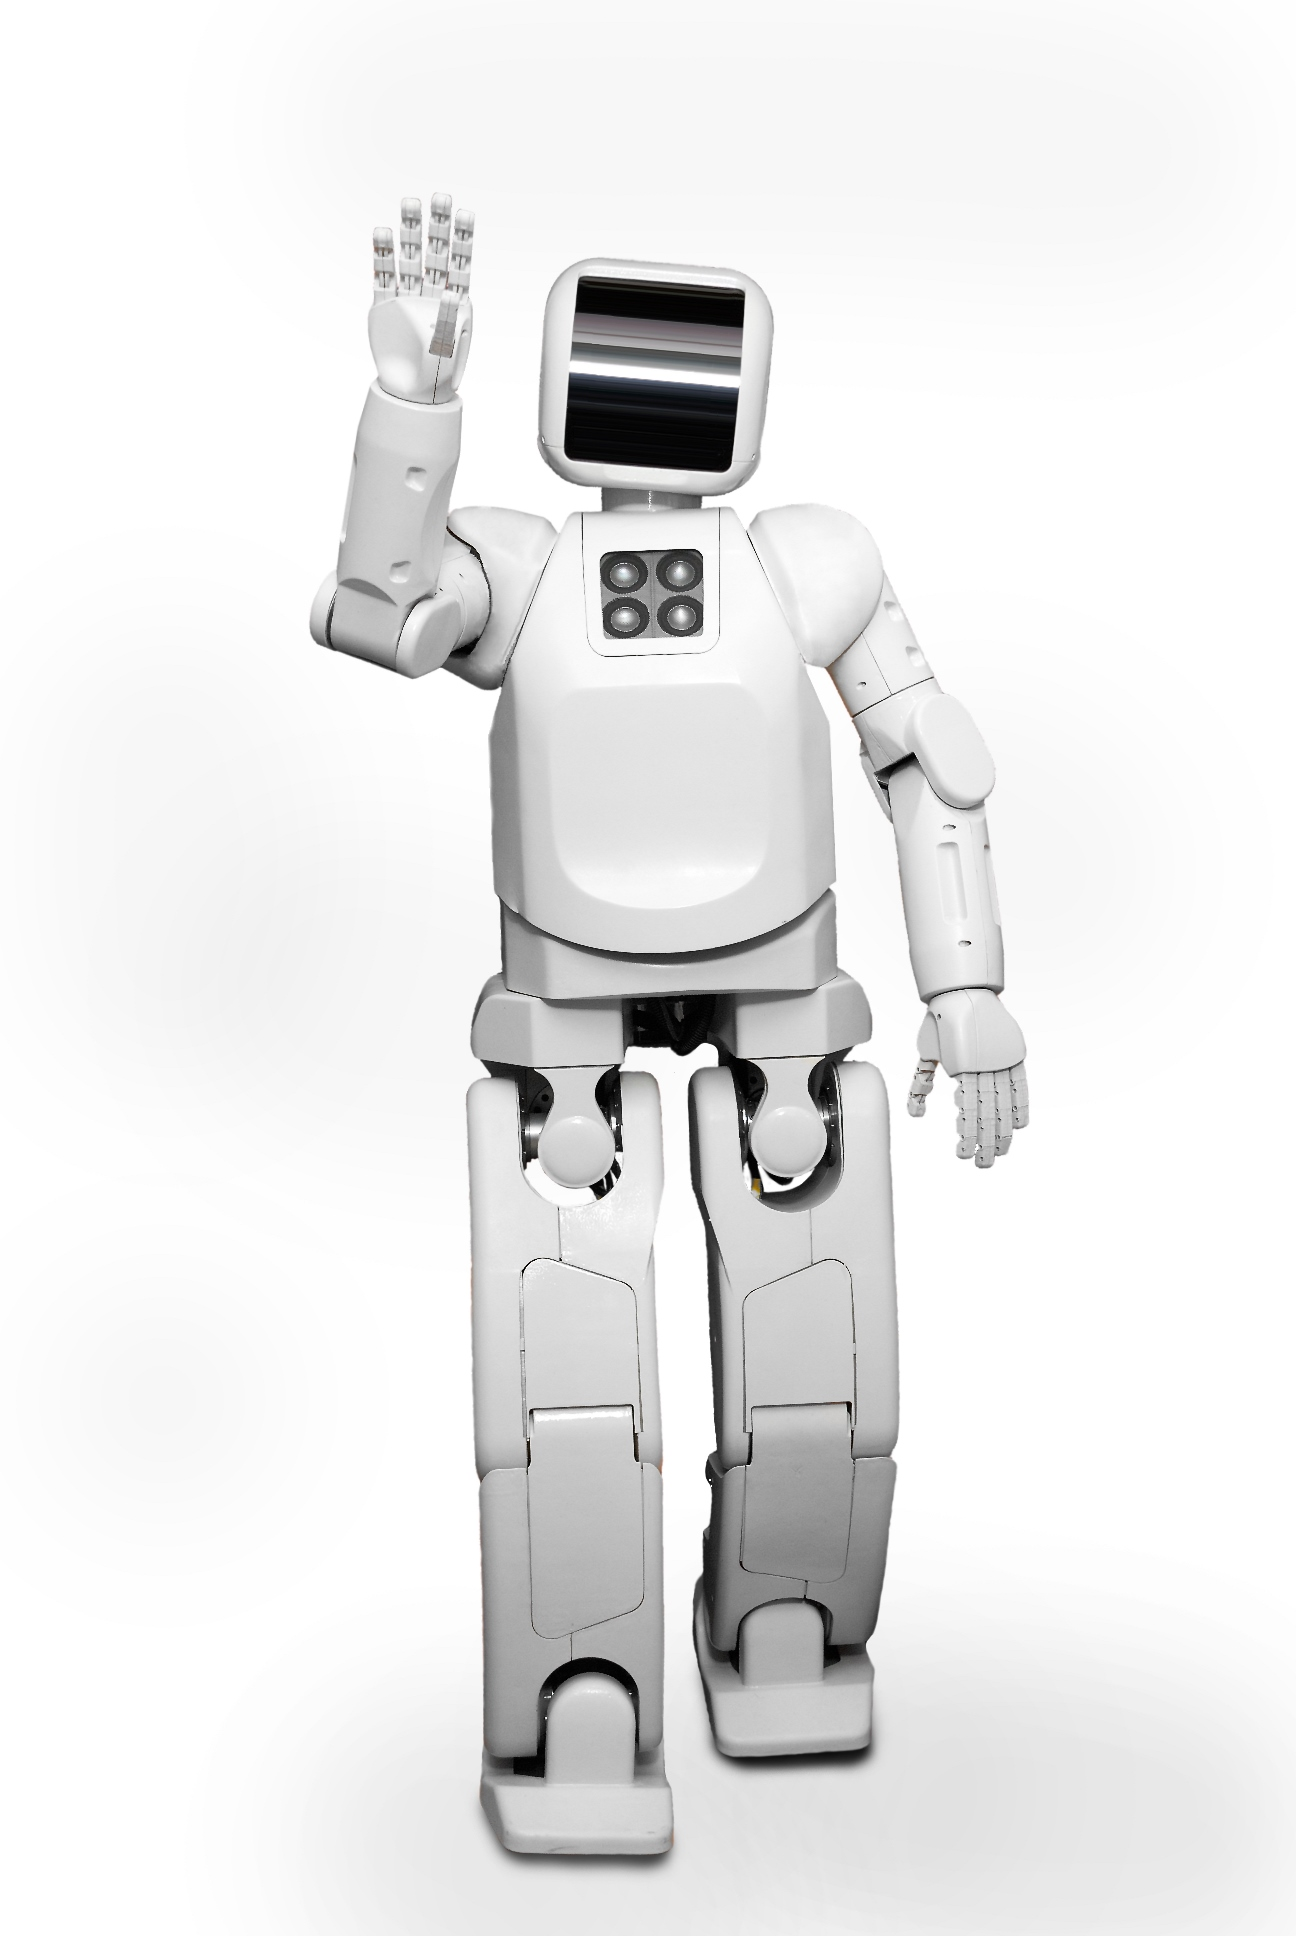
\includegraphics[scale=0.4]{ar600}}
      \caption{Antropomorphic robot AR-600.}
      \label{img:ar600}
\end{figure}


Abilities of robots to accomplish certain tasks autonomously relies mostly on
a high level software that implements all the best from the field of artificial
intelligence. The other way that allows to use robots now is to make them mimic
our moves like avatars. Presented AR-600 robot can be controlled by a developed
mimicking device (fig. \ref{img:suit}). It sends joint angles to robot and
gets back force feedback and video stream. With this ``suit'' on an
operator can naturally control the upperbody of the robot and use it to manipulate tools in uninhabitable or hazardous environments (e.g. welding or screwing).

AR-600 is already used in 6 Russian universities as a robotics research
platform. Some of the research topics are object grasping and bipedal walking.

This paper describes specifications of the robot, software developed so far and
some future work.

\begin{figure} [thpb]
      \centering
      \framebox{
      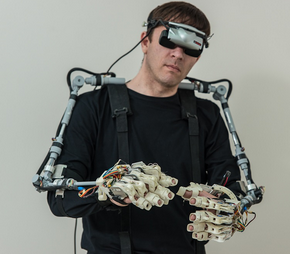
\includegraphics[scale=0.8]{suit}}
      \caption{Mimicking device for the robot.}
      \label{img:suit}
\end{figure}

\section{SPECIFICATIONS OF AR-600}

Height of the robot is 155 cm, its shoulder width is 38 cm, weight with
batteries is 54 kilograms.

Robot has 36 degrees of freedom (see table \ref{tbl:DOFTable}) with 13 degrees
of freedom in lower part including legs and pelvis and 5-DOF hands. Head with sensors has 3 DOF. Palm assemblies have 5
fingers with 1 degree of freedom each.
The overview of kinematic structure is shown in Fig.\ref{img:kinematic}.

 \begin{figure}[thpb]
      \centering
      \framebox{
        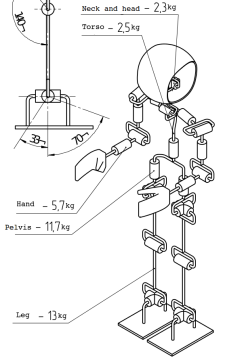
\includegraphics[scale=.5]{panview}
      }
      \caption{AR-600 kinematic scheme}
      \label{img:kinematic}
   \end{figure}
 

\begin{table}[thpb]
    \caption{Joints degrees of freedom (excluding palms)}
    \label{tbl:DOFTable}
    \begin{center}
    \begin{tabular}{c | c c c}
        & degree of freedom & range of motion, deg & \\
    \hline
        head & roll & -15 & 15 \\
            & tilt & -20 & 30 \\
            & pan & -90 & 90 \\
    \hline
        2 shoulders &  pitch & 0 & 105\\
                & yaw & -15 & 90\\
    \hline
        2 elbows & roll & -45 & +45 \\
                & flexion/extension & 0 & 130\\ 
    \hline
        2 wrists & roll & -45 & 45 \\
    \hline
        waist & yaw & -45 & 45 \\
    \hline
        2 hips & abduction/adduction & -11 & 20 \\
            & flexion/extension & 45 & -70 \\
            & rotation &-20 & 20\\
    \hline
        2 knees & rotation & -140 & 0 \\
    \hline
        2 ankles & flexion/extension & -33 & 70 \\
            & abduction/adduction & -20 & 11\\            
    \end{tabular}
    \end{center}
\end{table}

In order to place center of mass as close to hip joints as possible while
carrying accumulator batteries in chest cage, aluminium and steel alloys were
used for inner structure elements to achieve balance of weight and
endurance.
Maxon motors actuate major joints through belt transmission and harmonic drive
reducers to obtain desired torque and movement speeds.

Hip joints have 3 degrees of freedom each, obtaining movements from belt
transmissions of drives. Three motors driving a hip assembly are
situated in leg segment and lower body, flexion/extension drive is situated
in leg segment, other two are situated in pelvis segment.

Elbow joints are composed of two motors each - rotation motor assembly, directly
attached to Harmonic drive reducer, and flexion belt-transmission, placed
directly in joint axis (fig. \ref{img:joints}).
Ankle assembly has one belt transmission motor and motor, directly connected
to harmonic drive.
Shoulder joint assembly has 2 degrees of freedom, with both axes actuated by
toothed belt transmission.
Head assembly has a 3-DOF joint powered by brushed
motors in order to observe environment.
Exterior parts are made from 3D-printed plastic parts painted white.

\begin{figure}[thpb]
\centering
\framebox{
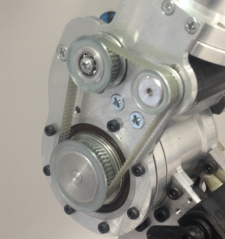
\includegraphics[scale=.5]{ElbowAssembly}}
\caption{Elbow assembly}
\label{img:joints}
\end{figure}

\begin{figure}[thpb]
\centering
\framebox{
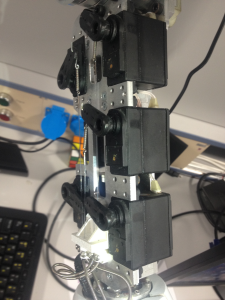
\includegraphics[scale=0.48]{wrist}}
\caption{Palm assembly}
\label{img:wrist}
\end{figure} 

Robot has palms with five fingers, one is opposite to another four. All
finger motors are placed in wrist-elbow section, Motor movements are
translated to fingers via system of strings (fig. \ref{img:wrist}). This system
limits wrist rotation, but makes whole assembly significantly lighter. This arm
is capable of grabbing objects like tennis ball, coffee cup or screw. However the next
version of hand is going to be more powerful. It will be released soon - palm
assembly is under constant development.

On-board PC is placed in the back of the robot. It is Avalue ECM-QM78 with Intel
Core i7-4700EQ CPU and 8GB RAM, capable of carrying out performance-demanding
sensor-processing tasks. 

Main controller board is built on top of 3 STM 32F107 microcontrollers, minor
driver controllers are built on STM 32F103 microcontrollers. Placement of
controller boards is shown on fig. \ref{img:electronics}.  All controllers use
Cortex-M3 ARM CPUs and provide software interfaces for hardware interaction.

\begin{figure}[thpb]
\centering
\framebox{
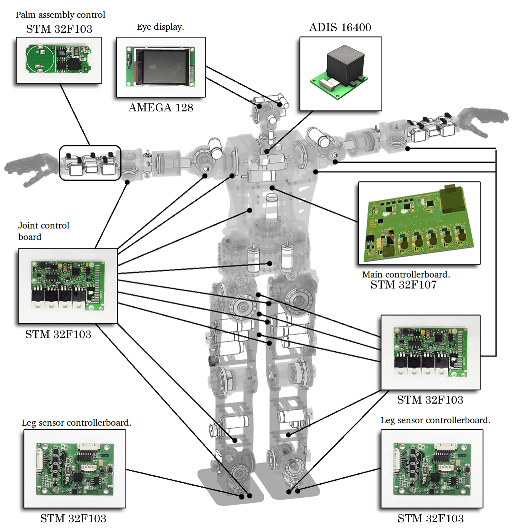
\includegraphics[scale=.67]{controllers}}
\caption{Controller boards}
\label{img:electronics}
\end{figure}

Joint drives are accompanied by two encoders. Main encoder provides absolute
position data with quite a broad error rate, supplementary encoder provides
relative motion data for more accurate position estimation.
 
Robot is equipped with CCD camera, speakers, microphone, pressure sensors
on its feets and fingertips and proximity sensors in hands. As an IMU an Analog
Devices ADIS 16400 is used, it is placed just in the center of mass. This point is considered as a base point of the robot. 

Additional sensors like Kinect or laser range finders could be placed in chest
frame. Two small displays in headmount mimic eyes and eyebrows.

AR-600 can run on internal LiFePo cells battery as well as on external power
source. Main voltage is 48V, individual parts operate with 6V, 8V and 12V.
Autonomous work time depends on many factors, but typically robot can run for a
30-40 minutes.

Internal communications are built on Ethernet. Controller boards are connected
via Zigbee interfaces to a switch, which governs internal network as shown
in fig. \ref{img:network}.

\begin{figure}[thpb]
\centering
\framebox{
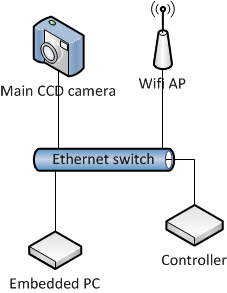
\includegraphics[scale=.5]{EthernetBus}}
\caption{Internal network scheme}
\label{img:network}
\end{figure}  

\section{SOFTWARE}

Main software interface for controller boards is UDP with specially formed
datagrams. There are two types of datagrams - one is for commands transmission,
another returns sensors data. Both UDP streams are independent.

\begin{figure}[thpb]
\centering
\framebox{
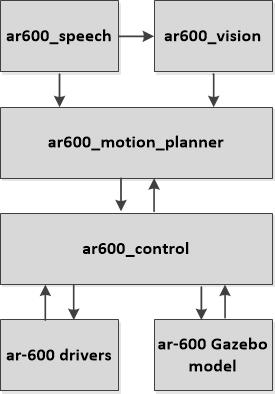
\includegraphics[scale=.7]{software}}
\caption{AR-600 software architecture.}
\label{img:software}
\end{figure}

\begin{figure}[thpb] 
\framebox{
\begin{minipage}[h]{0.49\linewidth}
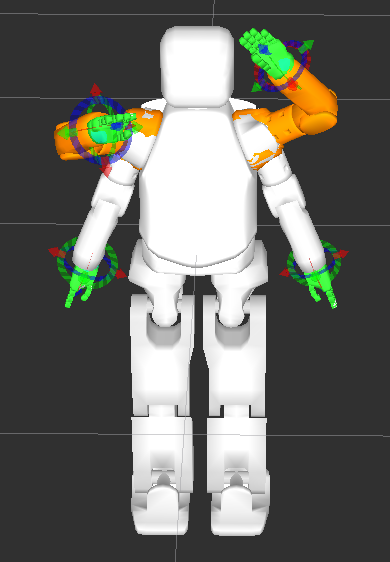
\includegraphics[scale=.25]{moveit}
\end{minipage}
\hfill
\begin{minipage}[h]{0.49\linewidth}
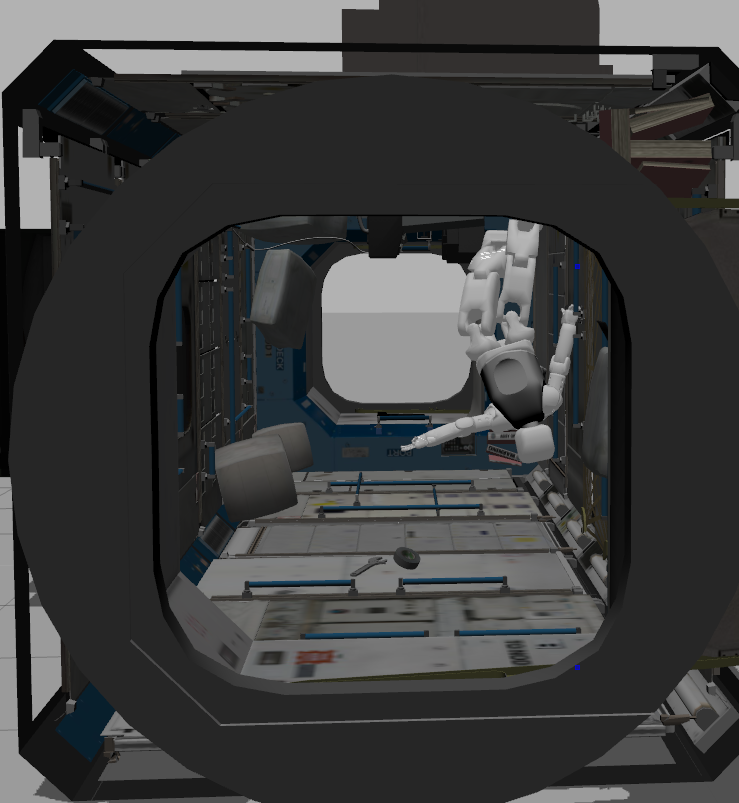
\includegraphics[scale=.155]{gazebo}
\end{minipage}
}
\caption{MoveIt demo and Gazebo simulation of AR-600}
\label{img:moveitgazebo}
\end{figure}

Datagram types encapsulate specific byte arrays, which encode movement
commands and sensors data, so anyone can easily interact with robot via standard
socket interface libraries.

Support for Robot Operating System \cite{c2} is a key to make the robot
available to the community and to benefit from open-source software. Not
reinventing the wheel and applying ready-to-use navigation and planning
solutions significantly increase speed of research and development for robotics
laboratories that work with AR-600.

AR-600 software architecture is shown on fig. \ref{img:software}. Crossplatform
drivers and ros\_control interface were implemented alongside with Rviz and
Gazebo models (see fig. \ref{img:moveitgazebo}). Motion planning is based on MoveIt! package \cite{c3} that uses state-of-the-art planning libraries. One can test planning
and obstacle avoidance for robot's limbs. Full body motion planner is under
development. Ar600\_vision package is capable of detecting, recognizing and
tracking human faces. Its implementation is based on cascade classifiers and
OpenCV library \cite{c4}. Ar600\_speech package lets the robot engage in
dialogue with people, answer simple predefined questions and execute motion or vision
commands. Pocketsphinx engine \cite{c5} developed by CMU is used as a core of
speech recognition for AR-600. ROS packages for the robot are not available for
public yet, but they are expected to be released soon.

\section{CONCLUSIONS}

This paper presented a humanoid robot AR-600, its hardware design and
specifications. Drivers and software that work under ROS framework are
also described.

The next generation of the robot, named AR-600E (fig. \ref{img:ar600e}) is
expected to be available soon and this will be more powerful, more lightweight,
more autonomous system.

Future work includes releasing ROS support packages for public use, development
of full-body motion planning with MoveIt (including bipedal walking). Switching
from position controller to torque controller is also a priority that
will enable more gentle and human-like moves. 

We hope AR-600 and his successor AR-600E will be among top humanoid platforms
used in robotics research and capable of working alongside with humans.

\begin{figure} [thpb]
      \centering
      \framebox{
      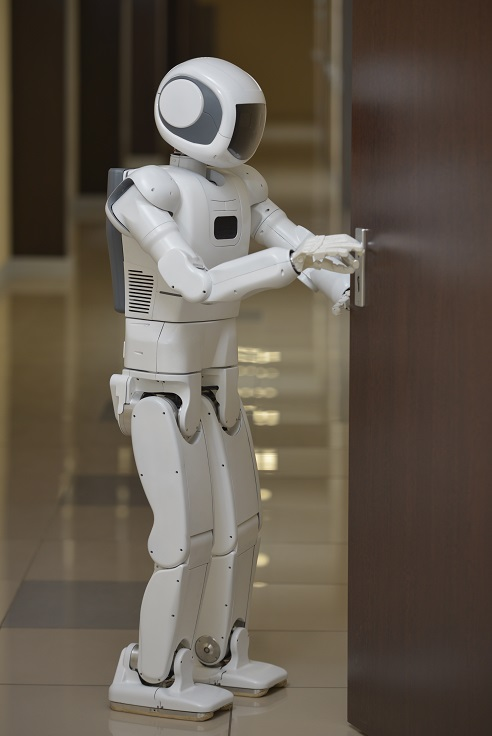
\includegraphics[scale=1]{ar600e}}
      \caption{AR-600E robot}
      \label{img:ar600e}
\end{figure}

\addtolength{\textheight}{-12cm}   % This command serves to balance the column lengths
                                  % on the last page of the document manually. It shortens
                                  % the textheight of the last page by a suitable amount.
                                  % This command does not take effect until the next page
                                  % so it should come on the page before the last. Make
                                  % sure that you do not shorten the textheight too much.

%%%%%%%%%%%%%%%%%%%%%%%%%%%%%%%%%%%%%%%%%%%%%%%%%%%%%%%%%%%%%%%%%%%%%%%%%%%%%%%%



%%%%%%%%%%%%%%%%%%%%%%%%%%%%%%%%%%%%%%%%%%%%%%%%%%%%%%%%%%%%%%%%%%%%%%%%%%%%%%%%



%%%%%%%%%%%%%%%%%%%%%%%%%%%%%%%%%%%%%%%%%%%%%%%%%%%%%%%%%%%%%%%%%%%%%%%%%%%%%%%%


\begin{thebibliography}{99}

\bibitem{c1} Android Techniques. URL: http://en.npo-at.com/
\bibitem{c2} M. Quigley, K. Conley, B. Gerkey, J. Faust, T. B. Foote, J. Leibs, R. Wheeler, and A. Y. Ng. ROS: an open-source robot operating system. In ICRA Workshop on Open Source Software, 2009.
\bibitem{c3} Ioan A. Sucan and Sachin Chitta, "MoveIt!", [Online] Available: http://moveit.ros.org
\bibitem{c4} G. Bradski. The OpenCV Library. Dr. Dobb’s Journal of Software
Tools (2000) 
\bibitem{c5} Huggins D. Daines, M. Kumar, A. Chan, et al. Pocketsphinx: A Free,
Real-Time Continuous Speech Recognition System for Hand-Held Devices Acoustics, Speech and Signal Processing, 2006. ICASSP 2006 Proceedings. 2006 IEEE International Conference on, Vol. 1 (2006)


\end{thebibliography}


\end{document}
